%%%%%%%%%%%%%%%%%%%%%%%%%%%%%%%%%%%%%%%%%%%%%%%%%%%%%%%%%%%%
%%  This Beamer template was created by Cameron Bracken.
%%  Anyone can freely use or modify it for any purpose
%%  without attribution.
%%
%%  Last Modified: January 9, 2009
%%
\def\crashsign#1{
	\begin{scope}[shift={#1}]%, rotate=#2]
		\draw [color=red!130!black, fill=red!20!black, very thick]
		(-0.15, -0.15) -- (0.15, 0.15);
		\draw [color=red!130!black, fill=red!20!black, very thick]
		(-0.15, 0.15) -- (0.15, -0.15);
	\end{scope}
}

\documentclass[xcolor=x11names,compress]{beamer}

%% General document %%%%%%%%%%%%%%%%%%%%%%%%%%%%%%%%%%
\usepackage{graphicx}
\usepackage{lmodern}
\usepackage{amsmath,bm}

\usepackage[babel,german=quotes]{csquotes}
\usepackage[backend=biber,style=alphabetic]{biblatex}
%\bibliography{bibliography.bib}

\usepackage{tikz}
\usetikzlibrary{arrows,shapes,automata,backgrounds,petri,positioning,calc}
%\usetikzlibrary{decorations.fractals}


\definecolor{myColor}{rgb}{0.73828125,0.1484375,0.203125}
%%%%%%%%%%%%%%%%%%%%%%%%%%%%%%%%%%%%%%%%%%%%%%%%%%%%%%

%\RequirePackage{filecontents}
%\begin{filecontents*}{bibliography.bib}
%@article{flp,
% author = {Fischer, Michael J. and Lynch, Nancy A. and Paterson, Michael S.},
% title = {Impossibility of Distributed Consensus with One Faulty Process},
% journal = {J. ACM},
% issue_date = {April 1985},
% volume = {32},
% number = {2},
% month = apr,
% year = {1985},
% issn = {0004-5411},
% pages = {374--382},
% numpages = {9},
%url = {http://doi.acm.org/10.1145/3149.214121},
% doi = {10.1145/3149.214121},
% acmid = {214121},
% publisher = {ACM},
% address = {New York, NY, USA},
%} 
%\end{filecontents*}




%% Beamer Layout %%%%%%%%%%%%%%%%%%%%%%%%%%%%%%%%%%
\useoutertheme[subsection=false,shadow]{miniframes}
\useinnertheme{default}
\usefonttheme{serif}
\usepackage{palatino}

\setbeamerfont{title like}{shape=\scshape}
%\setbeamerfont{frametitle}{shape=\scshape}
\setbeamerfont{caption}{size=\scriptsize}

\setbeamercolor*{lower separation line head}{bg=myColor} 
\setbeamercolor*{normal text}{fg=black,bg=white} 
\setbeamercolor*{alerted text}{fg=red} 
\setbeamercolor*{example text}{fg=black} 
\setbeamercolor*{structure}{fg=black} 

\setbeamercolor*{palette tertiary}{fg=black,bg=black!10} 
\setbeamercolor*{palette quaternary}{fg=black,bg=black!10} 

\setbeamertemplate{footline}[page number]
\setbeamertemplate{navigation symbols}{}
\setbeamertemplate{caption}[numbered]


\renewcommand{\(}{\begin{columns}}
\renewcommand{\)}{\end{columns}}
\newcommand{\<}[1]{\begin{column}{#1}}
	\renewcommand{\>}{\end{column}}
%%%%%%%%%%%%%%%%%%%%%%%%%%%%%%%%%%%%%%%%%%%%%%%%%%

\title{Automatic Brightness Adjustment}
\author{Lars Haulin, Robin Keller, Viktor Nordmark\\[1em] \textsc{\small{Uppsala Universitet}}}
\date{June 11, 2015}


\begin{document}
	\begin{frame}
		\titlepage
	\end{frame}
	
	
	%%%%%%%%%%%%%%%%%%%%%%%%%%%%%%%%%%%%%%%%%%%%%%%%%%%%%%
	%%%%%%%%%%%%%%%%%%%%%%%%%%%%%%%%%%%%%%%%%%%%%%%%%%%%%%
	\begin{frame}{Content}
		\tableofcontents
	\end{frame}
	
	%%%%%%%%%%%%%%%%%%%%%%%%%%%%%%%%%%%%%%%%%%%%%%%%%%%%%%
	%%%%%%%%%%%%%%%%%%%%%%%%%%%%%%%%%%%%%%%%%%%%%%%%%%%%%%
	\section{\scshape Motiviation}
	\subsection{}
	\begin{frame}{Concept}
		\begin{itemize}
			\item Hold fixed light intensity using
			\begin{itemize}
				\item Light bulb dimmer
				\item Light sensor
				\item Radio communication
			\end{itemize}
		\end{itemize}
		\begin{figure}
			\centering
			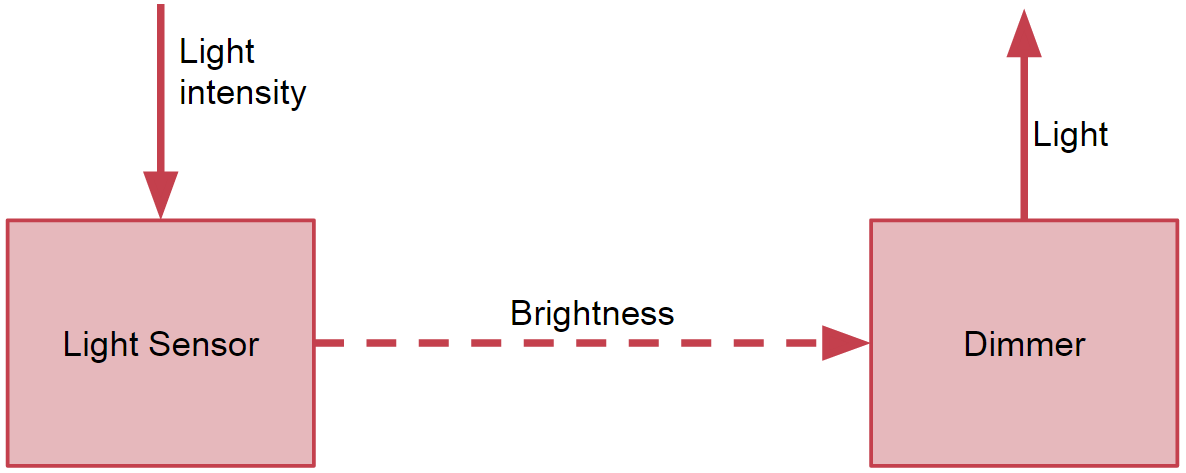
\includegraphics[width=0.8\textwidth]{data_flow.png}
			\caption{Data Flow}
		\end{figure}
	
		\note[item]{notes can go here}
	\end{frame}

	
	%%%%%%%%%%%%%%%%%%%%%%%%%%%%%%%%%%%%%%%%%%%%%%%%%%%%%%
	%%%%%%%%%%%%%%%%%%%%%%%%%%%%%%%%%%%%%%%%%%%%%%%%%%%%%%
	\section{\scshape Dimmer}
	\subsection{}
   \begin{frame}
      \Huge{\centerline{Dimmer}}
   \end{frame}

	\begin{frame}{Dimming Hardware and Software}
		\begin{itemize}
			\item Circuit
			\item How it works
			\item Theory
		\end{itemize}
		
	\end{frame}
	
	\begin{frame}{Circuit}
		
		\begin{figure}[ht!]
			\centering
			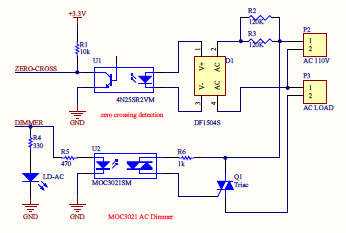
\includegraphics[width=0.8\textwidth]{Circuit.png}
			% \caption{Circuit}
			\label{fig:circuit}
		\end{figure} 
		
	\end{frame}
	
	\begin{frame}{Phase Control}
		
		\begin{figure}[ht!]
			\centering
			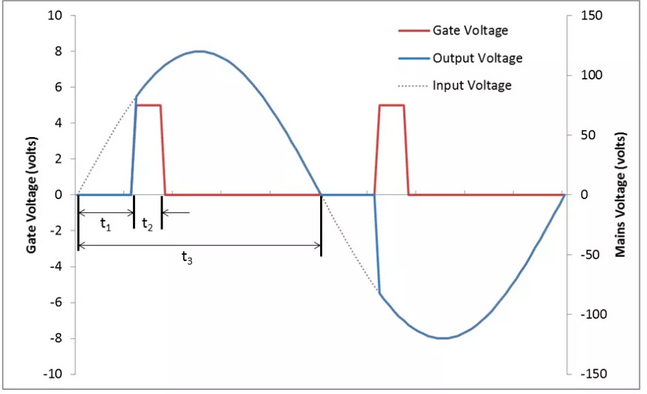
\includegraphics[width=0.8\textwidth]{Phase.png}
			% \caption{Circuit}
			\label{fig:circuit}
		\end{figure} 
		
	\end{frame}

	
	%%%%%%%%%%%%%%%%%%%%%%%%%%%%%%%%%%%%%%%%%%%%%%%%%%%%%%
	%%%%%%%%%%%%%%%%%%%%%%%%%%%%%%%%%%%%%%%%%%%%%%%%%%%%%%
	\section{\scshape Light Sensor Module}
	\subsection{}
   \begin{frame}
      \Huge{\centerline{Light Sensor Module}}
   \end{frame}

	\begin{frame}{Overwiew}
      \center
      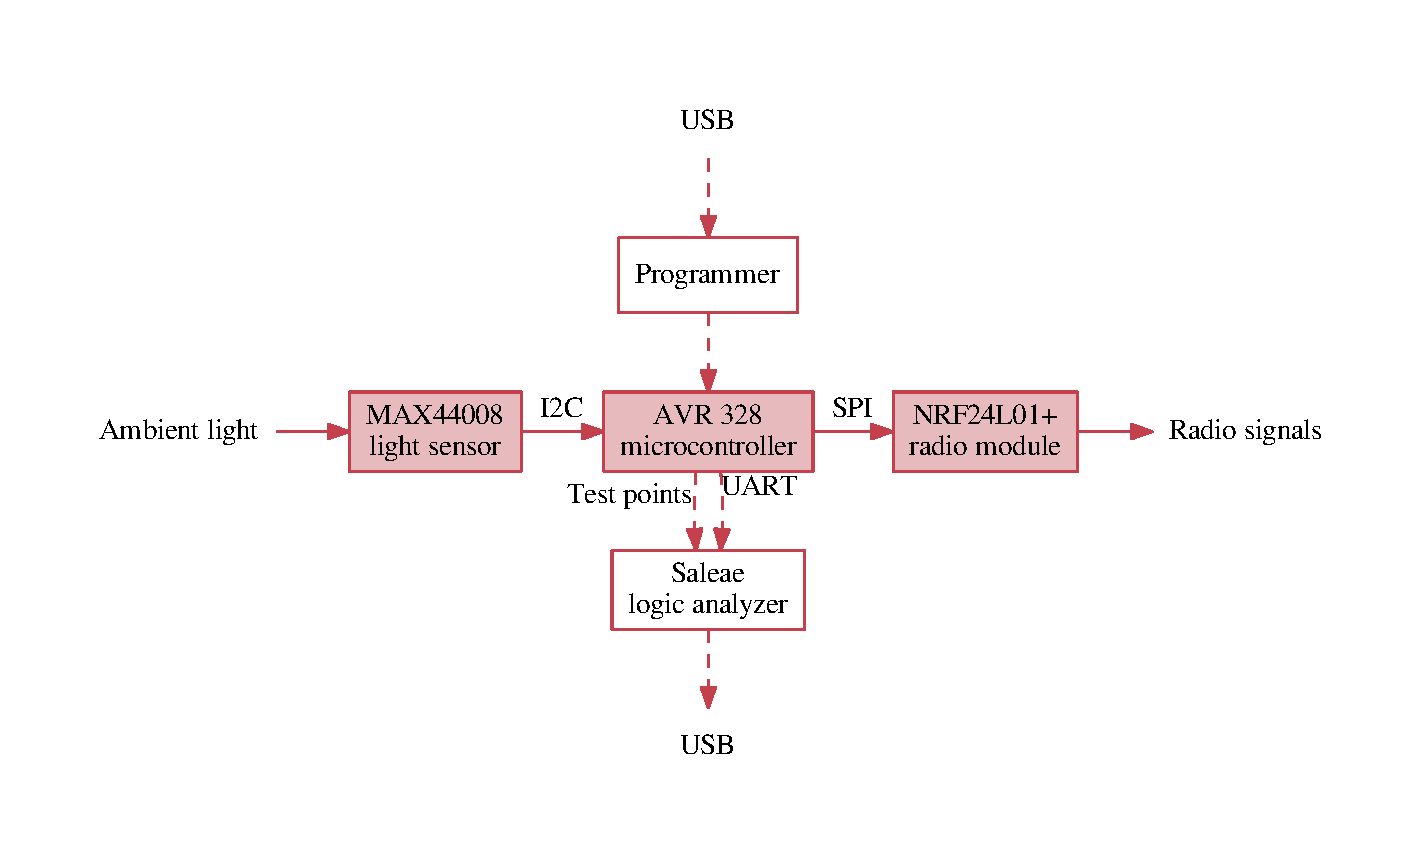
\includegraphics[width=1.1\textwidth]{sensorFlow.pdf}
	\end{frame}

	\begin{frame}{Sensor chip: MAX44008}
		Measures light, speaks I${}^2$C.

		Free sampling and shipping. It is tiny!
		\pause

		\centering
		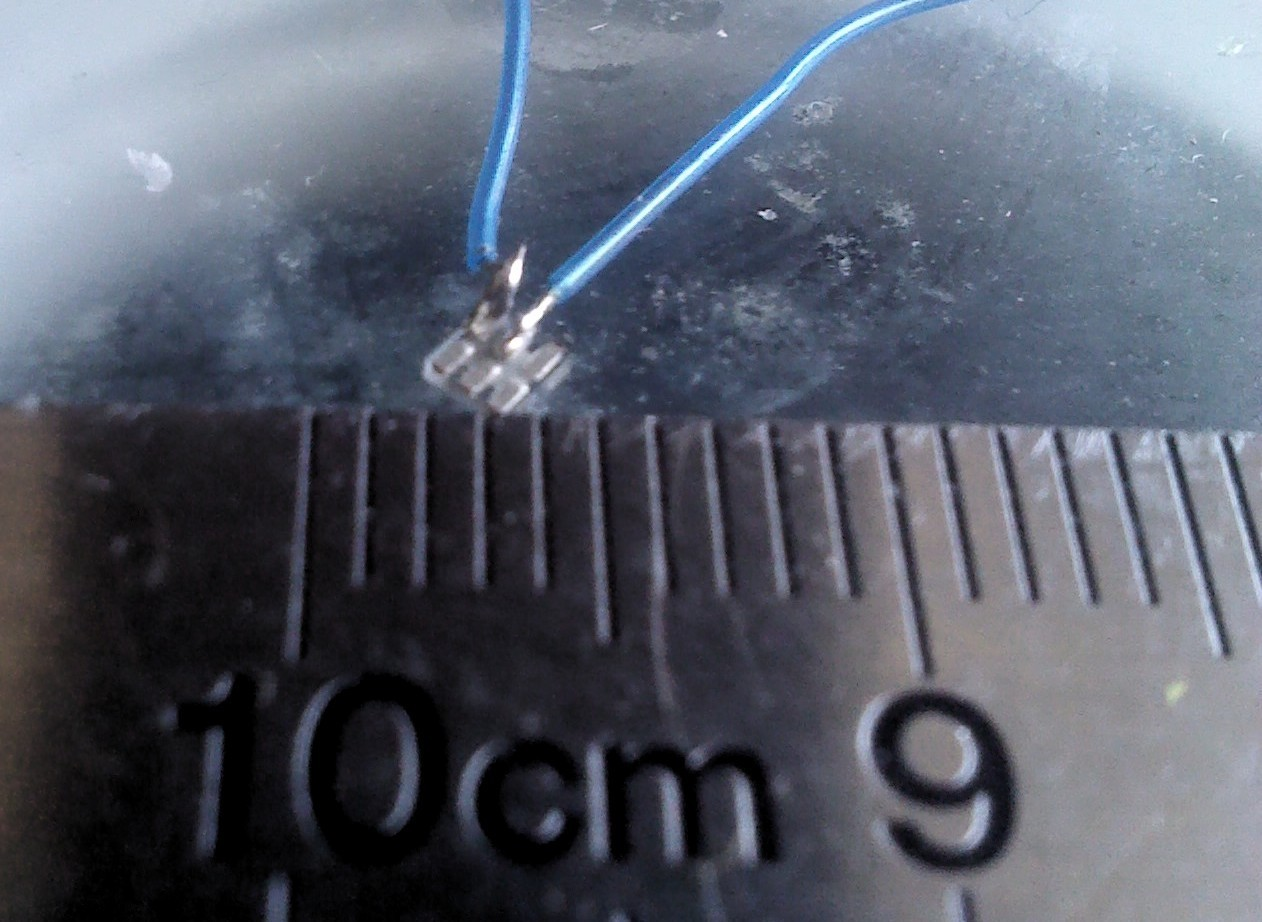
\includegraphics[width=0.8\textwidth]{sensorCables.jpg}
	\end{frame}

	\begin{frame}{First attempt}
		\centering
		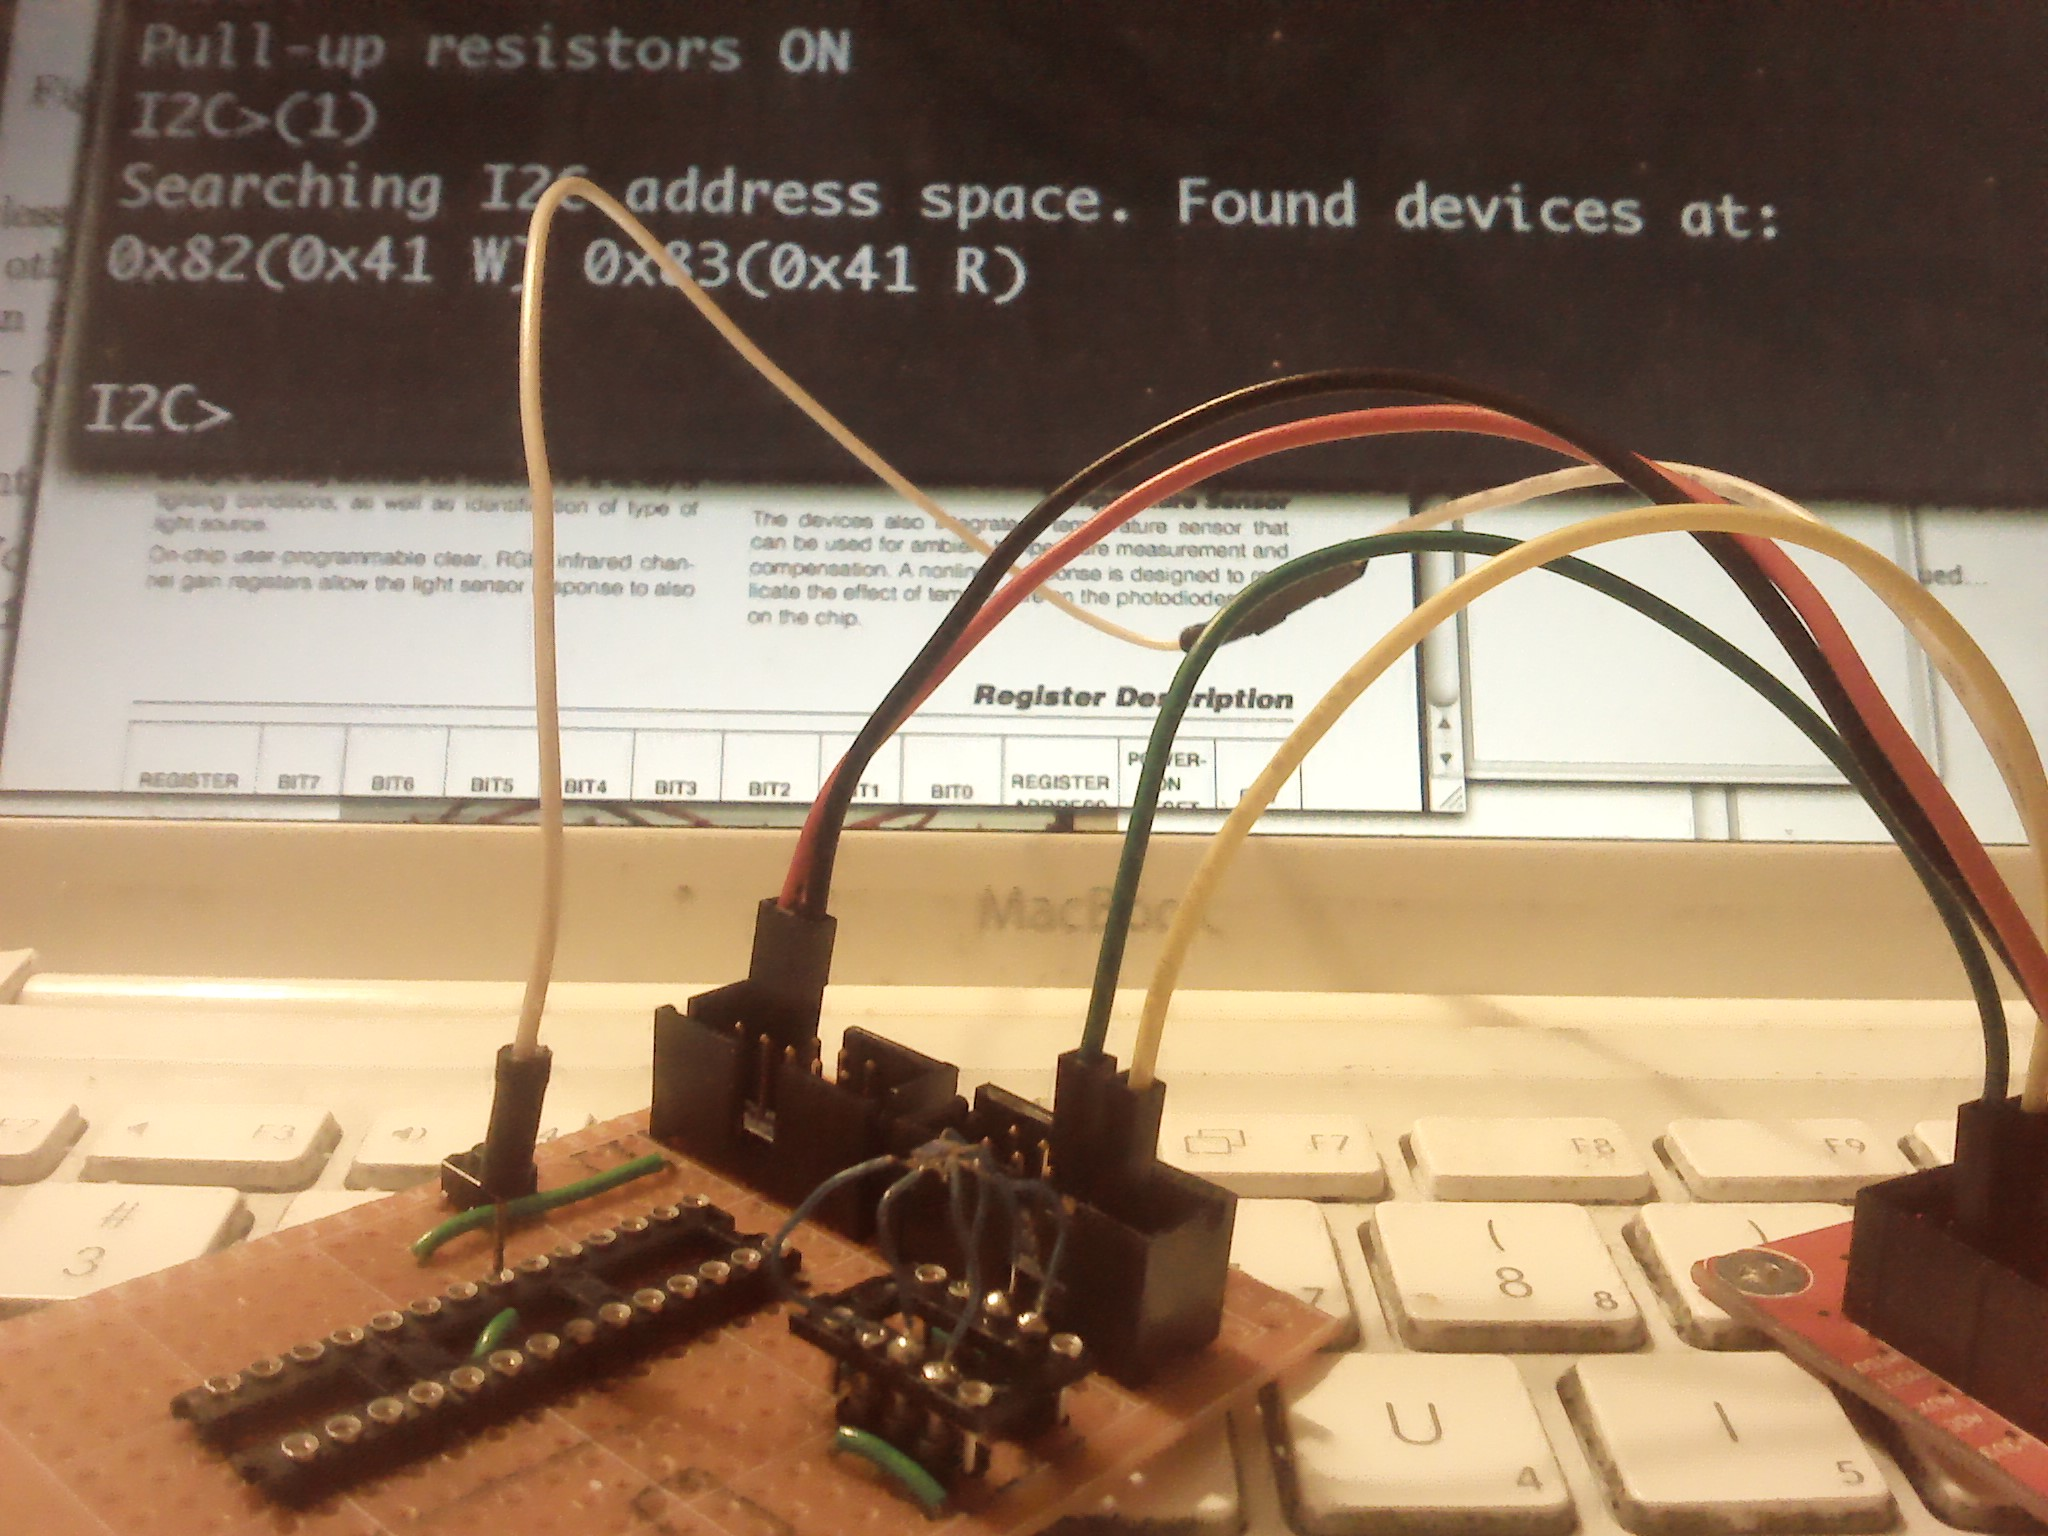
\includegraphics[width=0.8\textwidth]{buspirate.jpg}
	\end{frame}


	\begin{frame}{Checking analog signals}
		\centering
		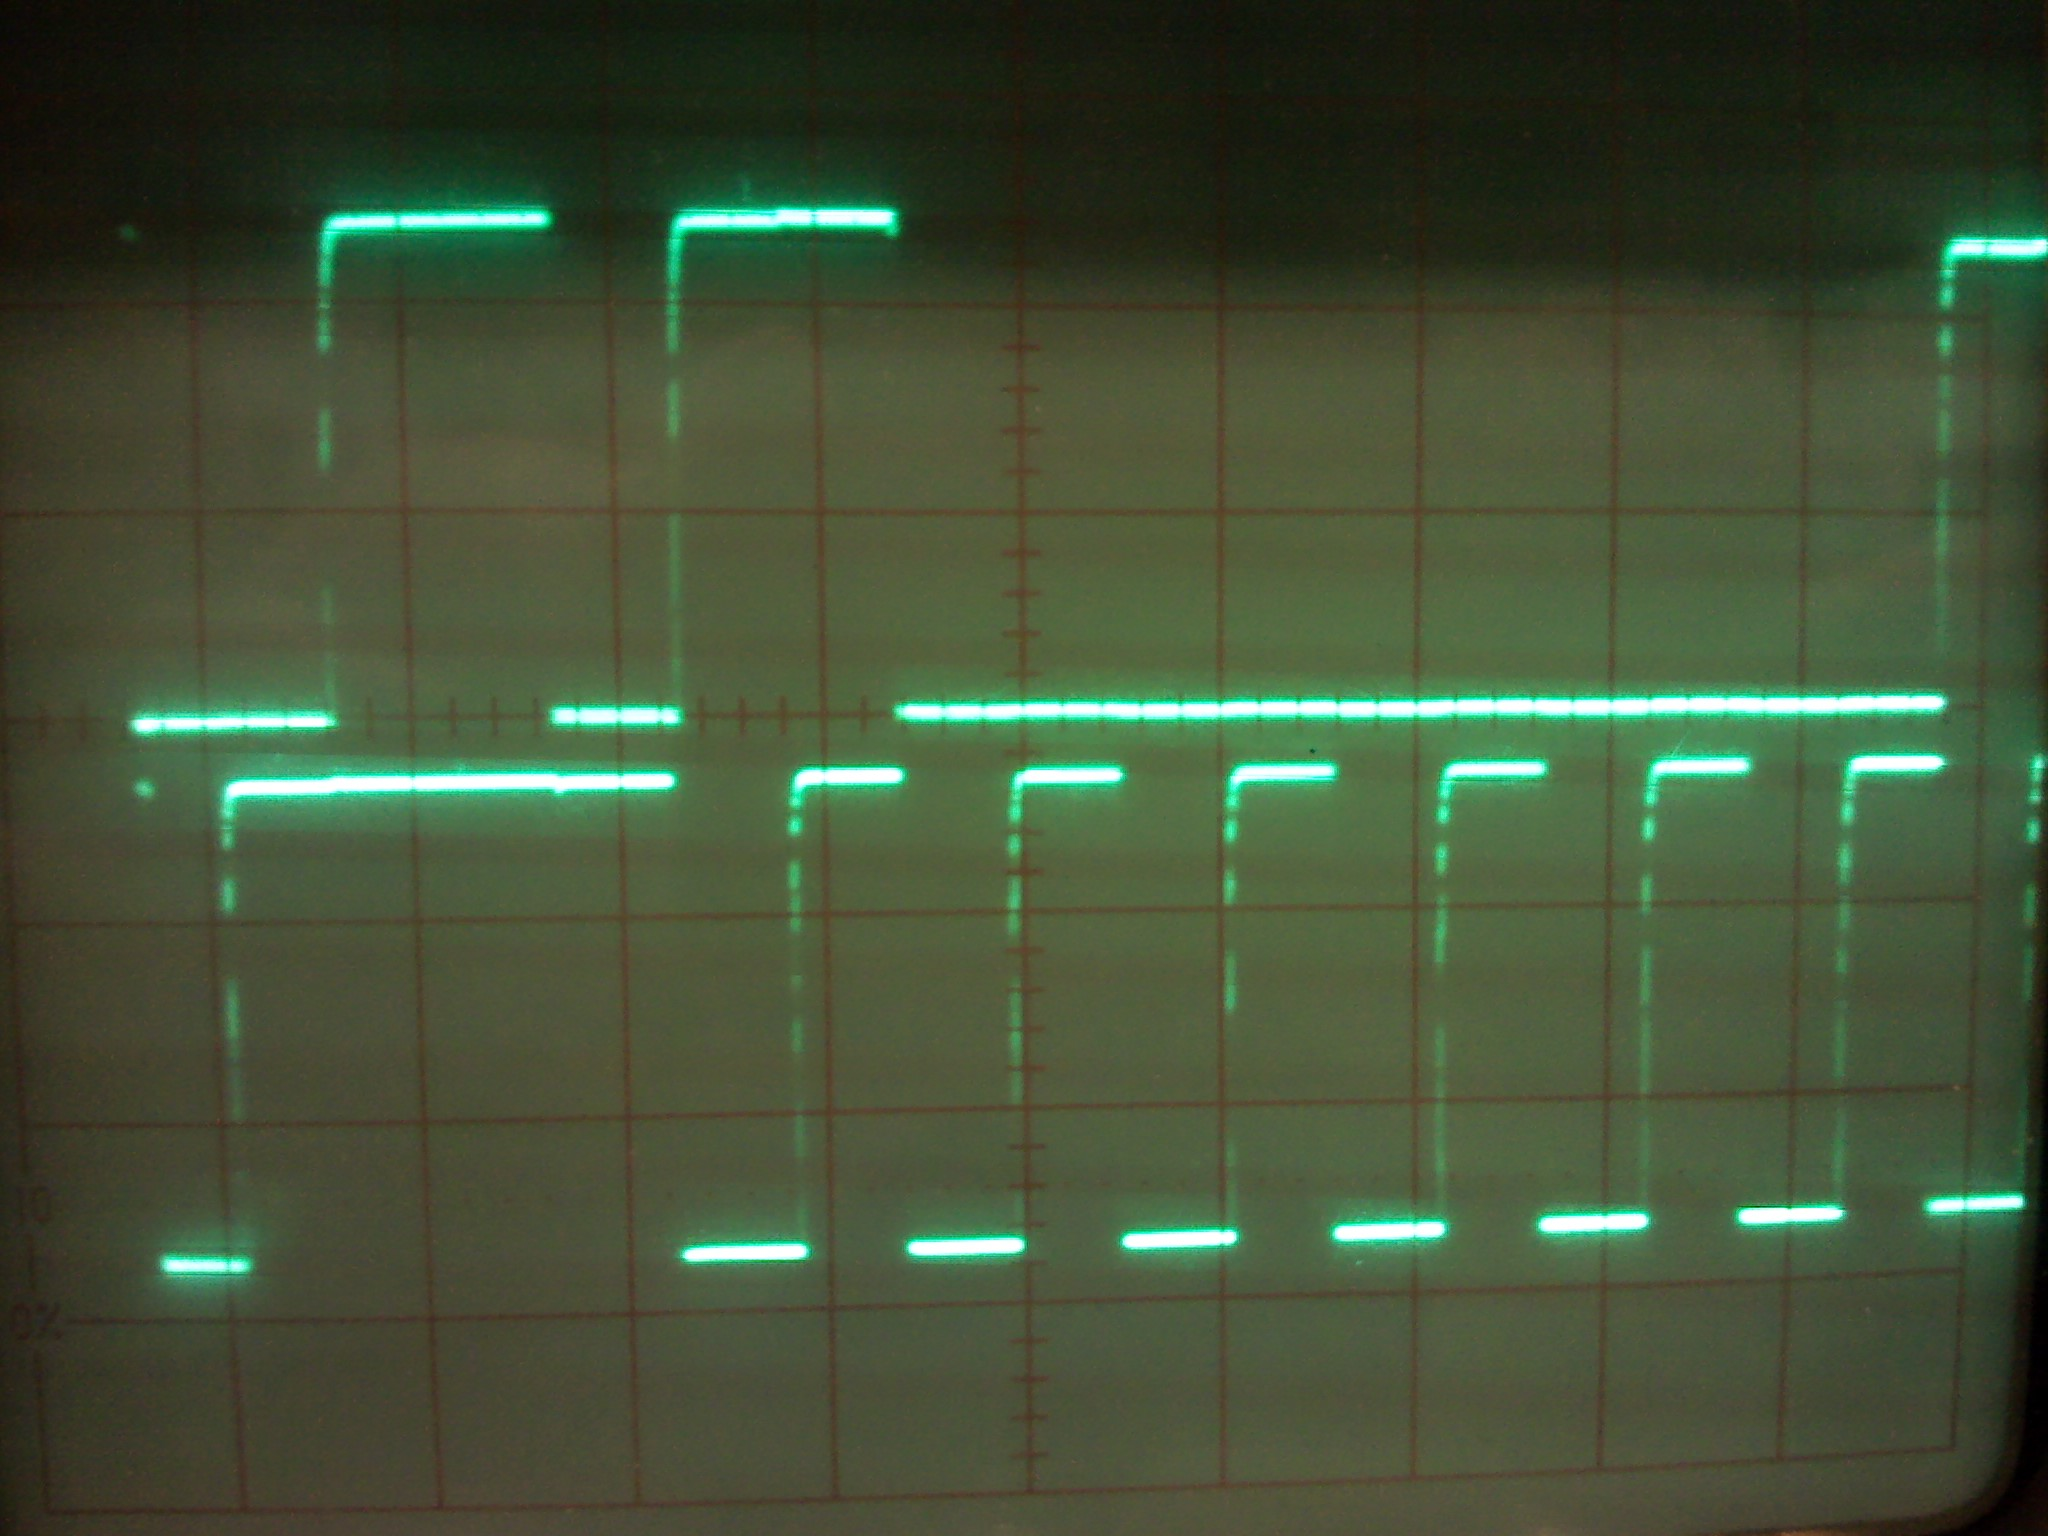
\includegraphics[width=0.8\textwidth]{oscilloscope.jpg}
	\end{frame}


	\begin{frame}{Etching Breakout board}
		\centering
		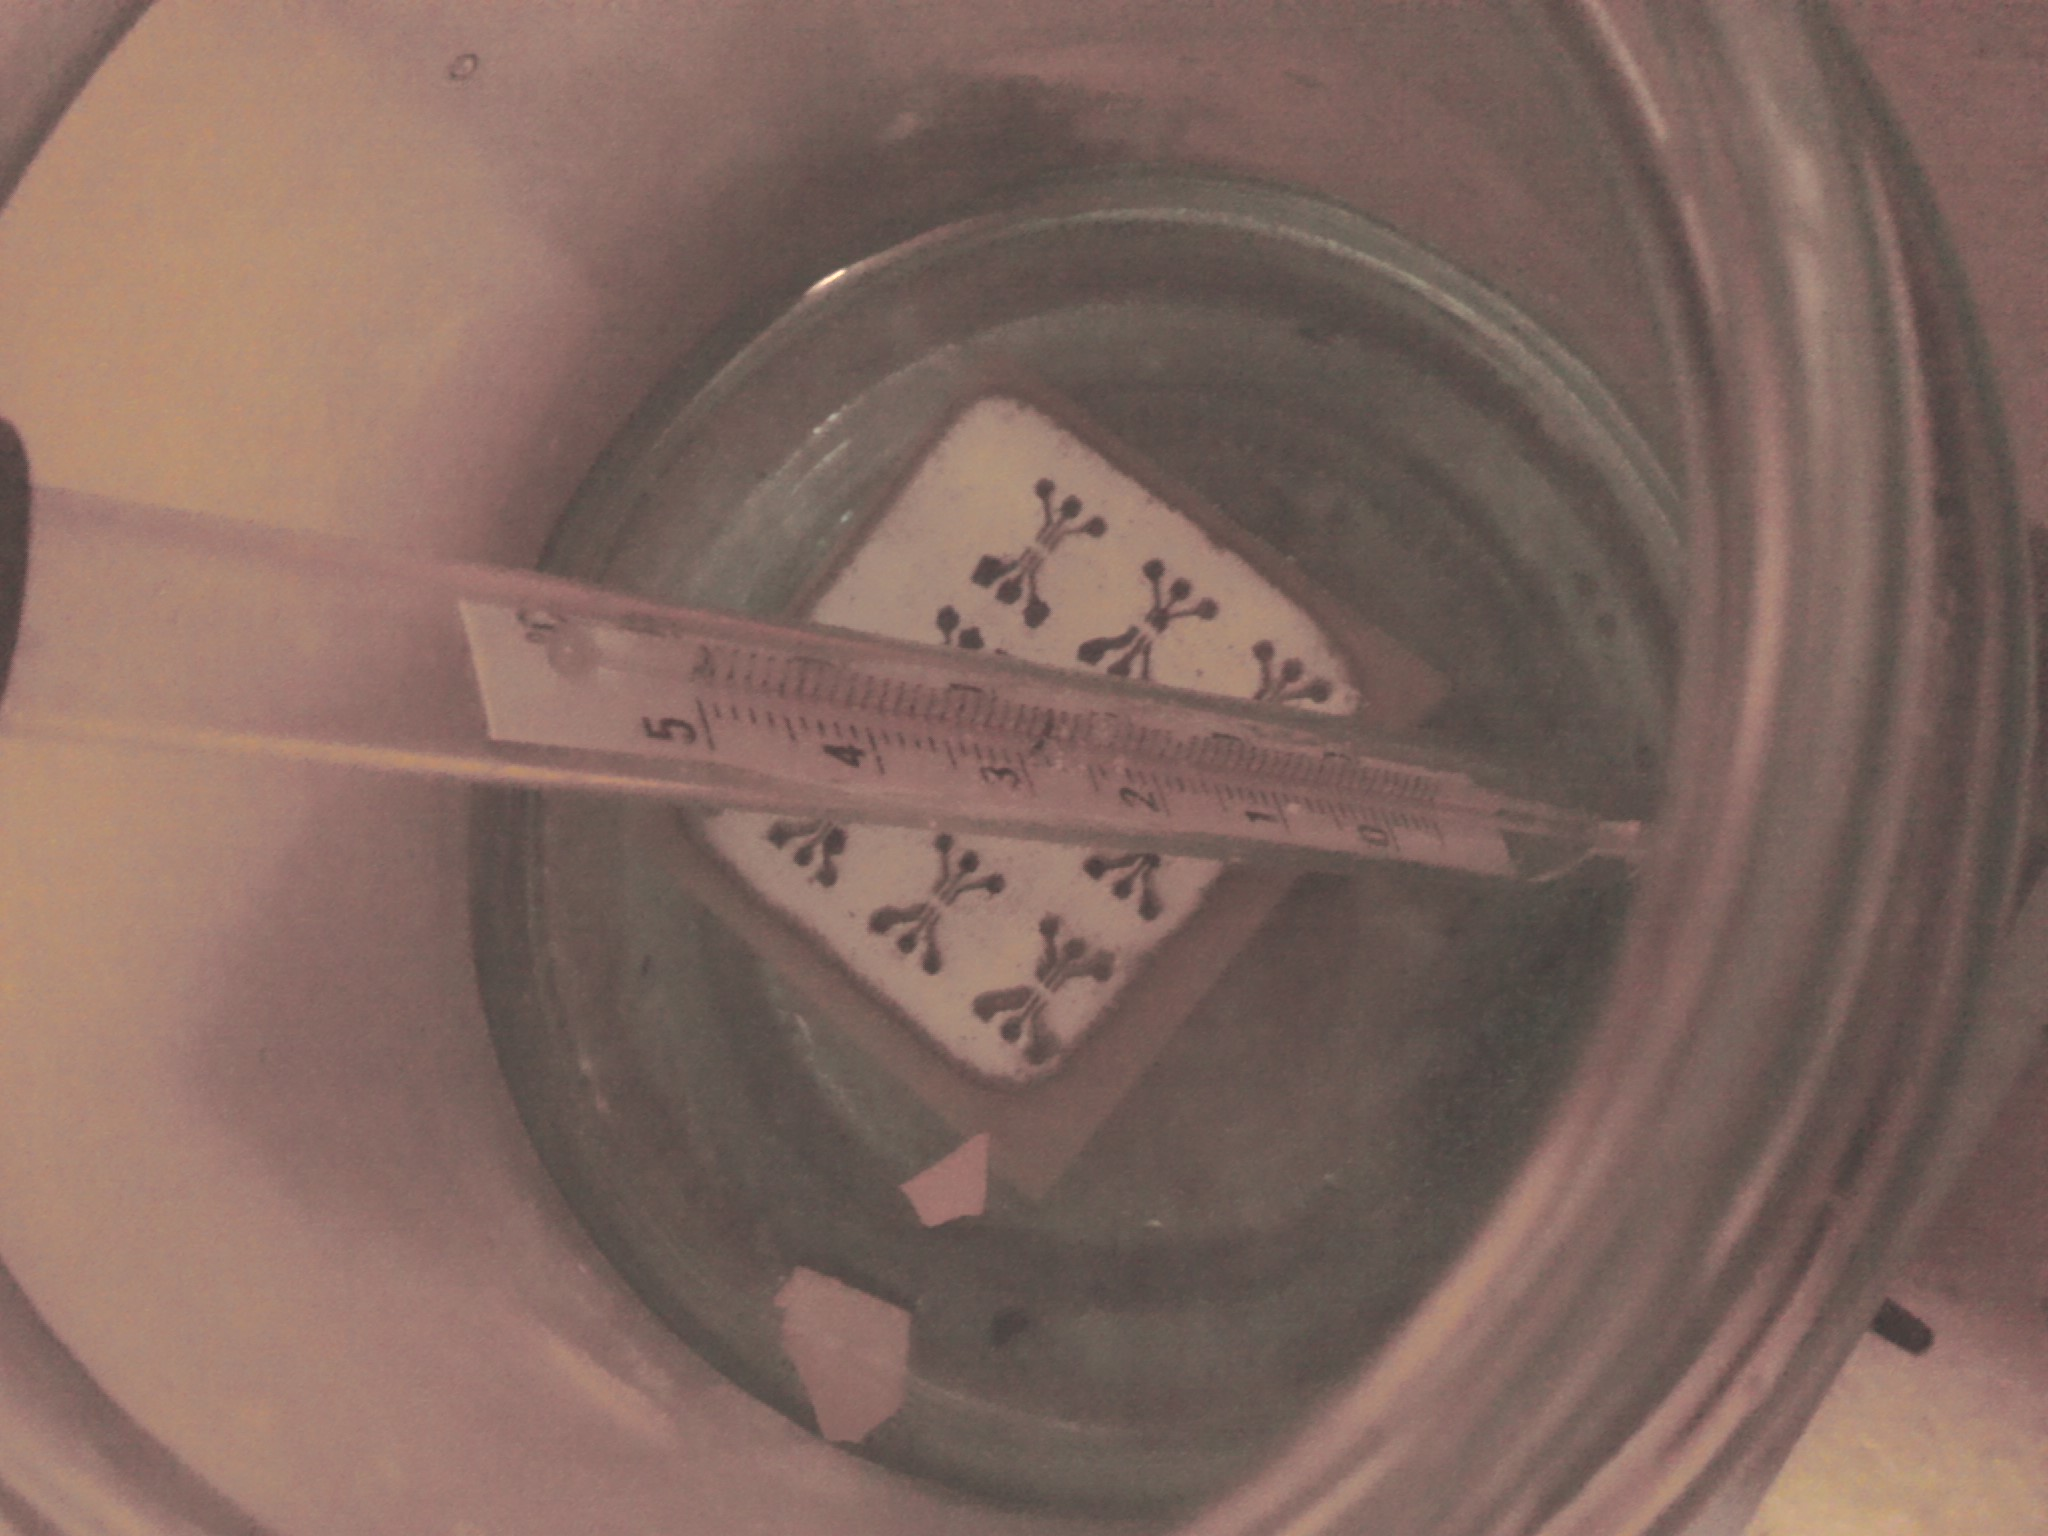
\includegraphics[height=0.5\textheight]{etching.jpg}
		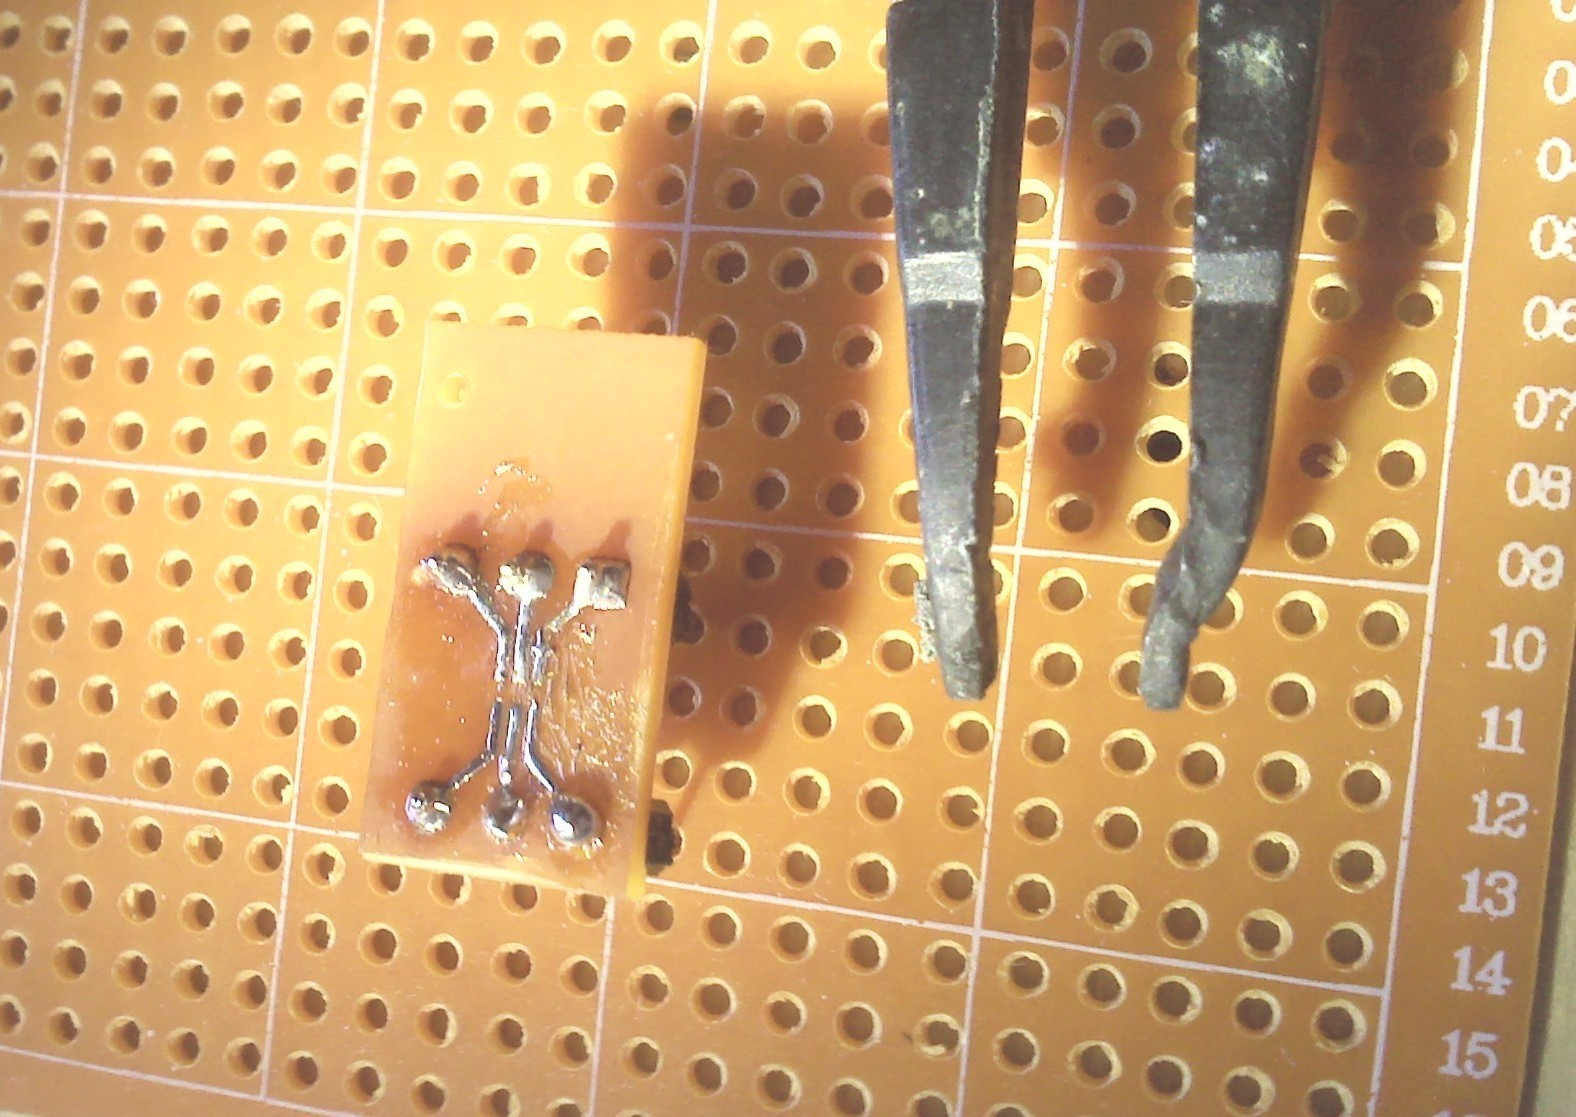
\includegraphics[height=0.5\textheight]{breakout.jpg}
	\end{frame}

	\begin{frame}{Logic signals}
		\centering
		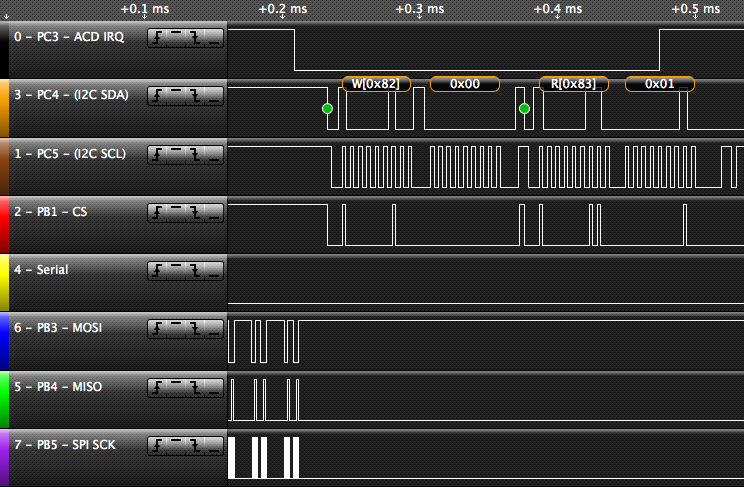
\includegraphics[width=0.8\textwidth]{logic.png}
	\end{frame}


	%%%%%%%%%%%%%%%%%%%%%%%%%%%%%%%%%%%%%%%%%%%%%%%%%%%%%%
	%%%%%%%%%%%%%%%%%%%%%%%%%%%%%%%%%%%%%%%%%%%%%%%%%%%%%%
	\section{\scshape Radio Communication}
	\subsection{}
   \begin{frame}
      \Huge{\centerline{Radio Communication}}
   \end{frame}

	\begin{frame}{Radio Communication using NRF24L01+}
		\begin{itemize}
			\item 2.4GHz, packet based messaging
			\item Communicate to radio module via SPI
			\item Maximum packet length of 32 Bytes
		\end{itemize}
	\end{frame}
	
	\begin{frame}{Radio Module Library}
		\begin{itemize}
			\item Each module gets a unicast and broadcast address
			\item Auto acknowledge for unicast packets
			\item Minimal interface
			\begin{itemize}
				\item Initializing, sending and receiving each function each
			\end{itemize}
		\end{itemize}
	\end{frame}
	
	
	%%%%%%%%%%%%%%%%%%%%%%%%%%%%%%%%%%%%%%%%%%%%%%%%%%%%%%
	%%%%%%%%%%%%%%%%%%%%%%%%%%%%%%%%%%%%%%%%%%%%%%%%%%%%%%
	\section{\scshape Conclusion}
	\subsection{}
	\begin{frame}{Difficulties}
		\begin{itemize}
			\item Current peaks of radio module
			\begin{itemize}
				\item Increase size of capacitor
			\end{itemize}
			\item Packaging of light sensor
			\item Explicit reset necessary to start radio module
			\begin{itemize}
				\item Set internal pullup for SPI
			\end{itemize}
			\item Reading value of light sensor
			\begin{itemize}
				\item Set acknowledge flag in I2C
			\end{itemize}
		\end{itemize}
	\end{frame}

	\begin{frame}{Live Demo}
		\begin{itemize}
			\item Live Demo
		\end{itemize}
	\end{frame}	
	
\end{document}
